\documentclass[
  american,aps,pra,reprint,floatfix,nofootinbib,superscriptaddress
]{revtex4-2}
% General document formatting
\usepackage{tikz}
\usepackage[margin=0.7in]{geometry}
\usepackage{xintfrac}
\usepackage{braket}
% Documentation:
% https://ftp.cc.uoc.gr/mirrors/CTAN/macros/latex/contrib/parskip/parskip.pdf
\usepackage[utf8]{inputenc}
\usepackage{hyperref}

% Math packages:
\usepackage{amsmath,amssymb,amsfonts,amsthm}

% Our definitions:
\DeclareMathOperator{\smoothen}{smoothen}
\DeclareMathOperator{\mean}{mean}
\DeclareMathOperator{\Tr}{Tr}
\DeclareMathOperator{\rank}{rank}
\DeclareMathOperator{\atantwo}{atan2}
\DeclareMathOperator{\real}{Re}
\DeclareMathOperator{\imag}{Im}
\DeclareMathOperator{\diag}{diag}
\DeclareMathOperator{\mspan}{span}
%\DeclareMathOperator{\arg}{arg}
\newcommand{\abs}[1]{\left|#1\right|}
\newcommand{\norm}[1]{\left\|#1\right\|}
\newcommand{\absmt}{\abs{m_{T}'}}
\newtheorem{theorem}{Theorem}
\newtheorem{lemma}[theorem]{Lemma}

% Draft comments
\usepackage{xcolor}
\newcommand{\VK}[1]{\textcolor{teal}{[VK: #1]}}
\newcommand{\DL}[1]{\textcolor{blue}{[DL: #1]}}
\newcommand{\NE}[1]{\textcolor{magenta}{[NE: #1]}}

\begin{document}

\title{Machine learning Fisher Information Metric from bitstrings}
\author{First Last}
\email{email}
\affiliation{USC affiliation}

\date{\today}

\begin{abstract}
We present a machine-learning based method ``Bitstring-ChiFc'' which,
given a dataset corresponding to a family of distributions of bitstrings
parameterized by a manifold, can produce a rough approximation
for the corresponding Fisher Information Metric.
We observe that for multiple toy models there are often enough simple patterns
in the data that this approach
achieves satisfactory approximation even for dataset sizes small
compared to the number of possible bitstrings.
\end{abstract}

\maketitle

\section{Introduction}
\DL{Give a general introduction to the problem we wish to solve and include pertinent background with citations. In particular, we need to address why people care about QPTS, what is the computational complexity of identifying QPTs, and why we think that having a QC can be helpful in this regard.}

\subsection{Challenge: finding phase transitions}
%%DL too colloquial
%Let's talk about phase transitions.  

\DL{Presentation of this Hamiltonian should come later, when we discuss a specific example. Or, you can use it in the introduction to motivate some of the specific questions we're attempting to answer, but then refer to it explicitly in terms of some specific aspects of the phase diagram.}

Consider the Hamiltonian
on a $2 \times L$ lattice given by the following equations.
\begin{equation}
  \label{eq:Hladder.1}
  H(s,K,U) = (1-s) H_0 + s H_1,
\end{equation}
\begin{equation}
  \label{eq:Hladder.2}
  H_0 = -\sum_{i=0}^{L-1} (X_{T_i} + X_{B_i}),
\end{equation}
\begin{multline}
  \label{eq:Hladder.3}
  H_1 = \sum_{i=0}^{L-1} \biggl(K Z_{T_i} Z_{T_{i+1}} - K Z_{T_i} Z_{B_i}
    - K Z_{B_i} Z_{B_{i+1}} \\
  - K Z_{T_i} + \frac{U}{2} Z_{B_i}\biggr).
\end{multline}
Here qubits $T_L$ and $B_L$ are identified with $T_0$ and $B_0$ respectively.

It is called ``Frustrated Ladder Hamiltonian'' and is schematically represented
by the following diagram:
\begin{center}
  \pgfmathparse{\columnwidth/10.7cm}%
  \edef\tikzscale{\pgfmathresult}%
  \begin{tikzpicture}[scale=\tikzscale]
    \foreach \x in {0,...,9}{
      \draw (\x,0) circle (0.3) node (n0x\x){$T_{\x}$};
      \draw (\x,-1) circle (0.3) node (n1x\x){$B_{\x}$};
      \draw (n0x\x) -- (n1x\x);
    }
    \foreach \x[count=\xnext from 1] in {0,...,8}{
      \draw[dotted,line width=1pt] (n0x\x) -- (n0x\xnext);
      \draw (n1x\x) -- (n1x\xnext);
    }
    \draw[dotted,line width=1pt] (-0.7,0) -- (n0x0);
    \draw (-0.7,-1) -- (n1x0);
    \draw[dotted,line width=1pt] (9.7,0) -- (n0x9);
    \draw (9.7,-1) -- (n1x9);
  \end{tikzpicture}
\end{center}
On this diagram of $L=10$ Frustrated Ladder Hamiltonian
the solid lines represent ferromagnetic couplings and
dotted lines --- antiferromagnetic couplings. For a fixed $L$
the Frustrated Ladder Hamiltonian depends on 3 parameters, $s, K, U$.
We set $K=1$ and consider the values $s\in[0,1]$, $U\in[0,1]$.

How would one find phase transitions of that Hamiltonian? For that particular
Hamiltonian people already know a couple of order parameters given by the
following equations.
\begin{equation}
  \label{eq:mt}
  \absmt = \abs{\sum_i Z_{T_i}(-1)^i}
\end{equation}
\begin{equation}
  \label{eq:mb}
  m_B = \sum_i Z_{B_i}
\end{equation}

These are called ``staggered magnetization of the top row'' and ``magnetization
of the bottom row'' respectively. We can compute these magnetizations for various
values of the parameters of the Hamiltonian for $L=10$ and produce the
following diagrams:

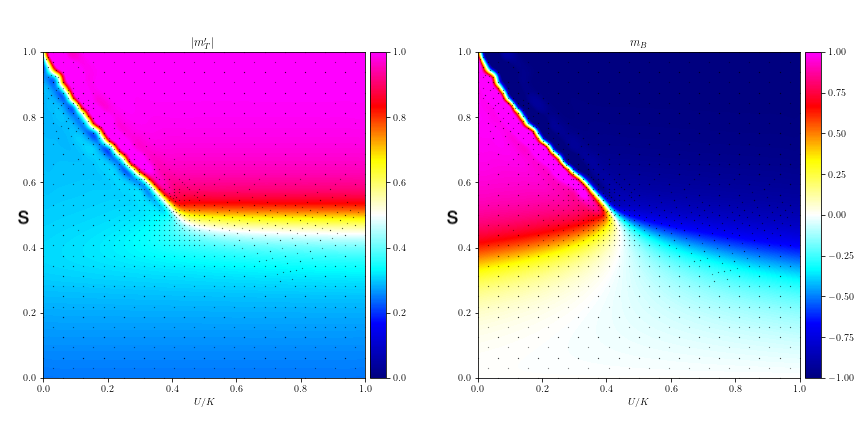
\includegraphics[width=\dimexpr\columnwidth-10.0pt]{lanczos_chi0_gp.png}

\VK{The following statement is in the direct contradiction with the statement
that the main goal of this paper is to learn Fisher Information Metric
given a dataset of bitstrings.}
In this work we focus on the task of identifying phase transitions in a
family of Hamiltonians $\{H_{\lambda}\}_{\lambda \in \Lambda}$ acting on a finite
set of qubits, and given access to an oracle capable -- given $\lambda \in \Lambda$ --
of producing bitstrings measured in the computational basis from a state sampled
from a low temperature distribution corresponding to the Hamiltonian
$H_{\lambda}$. 
%Specifically, 
\DL{The following sentence is very generic; it describes almost all attempts to demonstrate a quantum advantage. It can be moved to the very beginning of the introduction, or even deleted altogether.}
More generally,
the main goal of this paper is to make some
progress towards attempting to understand whether algorithms using
quantum computers can have an advantage over algorithms using the
same amount of resources but running on
purely classical hardware as illustrated in the following diagram.
\begin{center}
  \pgfmathparse{\columnwidth/13.37cm}%
  \edef\tikzscale{\pgfmathresult}%
  \begin{tikzpicture}[scale=\tikzscale]
    \newlength{\ux}
    \setlength{\ux}{15mm}
    \newlength{\uy}
    \setlength{\uy}{11mm}
    \draw (-3\ux, 0) node (H) {$\left\{H_\lambda\right\}$};
    \draw (0, 1.5\uy) node (A1)
      {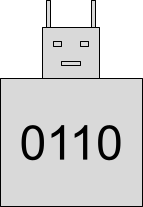
\includegraphics[width=0.15\columnwidth]{robot_classical.png}};
    \draw (0, -1.5\uy) node (A2)
      {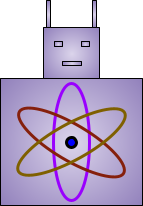
\includegraphics[width=0.15\columnwidth]{robot_quantum.png}};
    \draw (4\ux, 1.5\uy) node (B1)
      {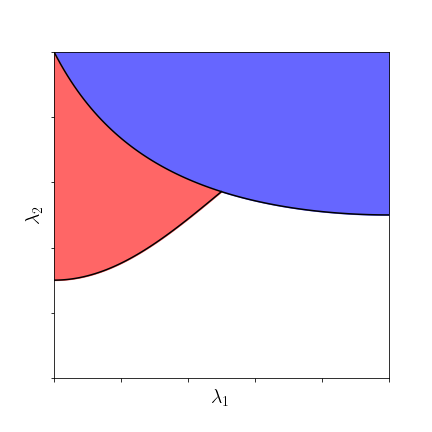
\includegraphics[width=0.28\columnwidth]{fake_phase_diagram.png}};
    \draw (4\ux, -1.5\uy) node (B2)
      {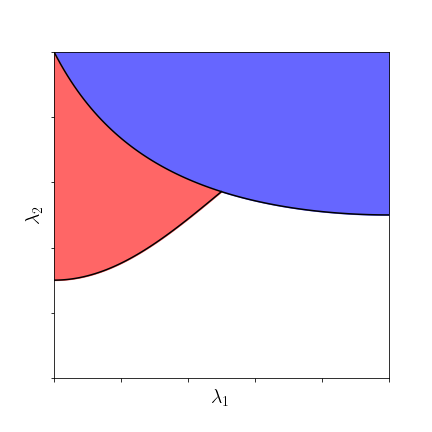
\includegraphics[width=0.28\columnwidth]{fake_phase_diagram.png}};
    \draw [->] (H.north) to[out=90,in=180] (A1.west);
    \draw [->] (H.south) to[out=-90,in=-180] (A2.west);
    \draw [->] (A1) -- (B1);
    \draw [->] (A2) -- (B2);
  \end{tikzpicture}
\end{center}
\VK{TODO: the idea of classical and quantum ``robots'' was taken from some
paper (probably Preskill). Find and cite that paper} \DL{yes: Fig.1 of https://www.science.org/doi/10.1126/science.abn7293}

More specifically, throughout this work we consider algorithms attempting
to take an advantage of quantum computer having a specific structure. First,
we use quantum annealer to generate a dataset of bitstrings measured
in the computational basis corresponding
to various values of the parameters. Then we use a classical algorithm
involving machine learning
to process those bitstrings into an estimates of where phase transitions
are located. We also allow for an interactive version of this structure
where the classical part of the algorithm can produce additional requests
(values of the parameters and counts of samples requested) for the quantum
annealer generating bitstrings.
\begin{center}
  \pgfmathparse{\columnwidth/13.37cm}%
  \edef\tikzscale{\pgfmathresult}%
  \begin{tikzpicture}[scale=\tikzscale]
    \setlength{\ux}{15mm}
    \setlength{\uy}{11mm}
    \draw (-3\ux, 0) node (H) {$\left\{H_\lambda\right\}$};
    \draw (0, 1.5\uy) node (A1)
      {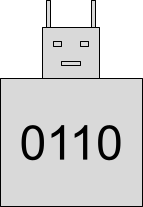
\includegraphics[width=0.15\columnwidth]{robot_classical.png}};
    \draw (-1.9\ux, -1.5\uy) node (A2a)
      {
\includegraphics[width=0.1\columnwidth]{qa.png}};
    \draw (-0.15\ux, -1.5\uy) node (A2b)
      {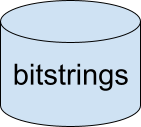
\includegraphics[width=0.15\columnwidth]{bitstrings.png}};
    \draw (1.6\ux, -1.5\uy) node (A2c)
      {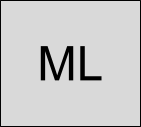
\includegraphics[width=0.1\columnwidth]{ml.png}};
    \draw (4\ux, 1.5\uy) node (B1)
      {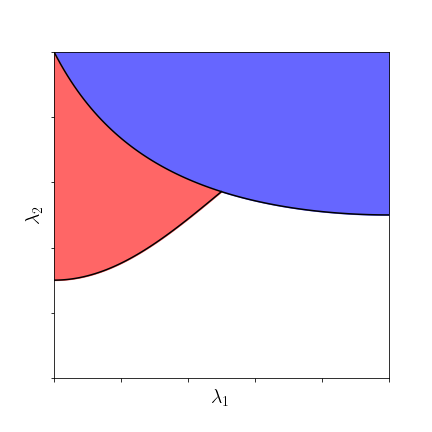
\includegraphics[width=0.28\columnwidth]{fake_phase_diagram.png}};
    \draw (4\ux, -1.5\uy) node (B2)
      {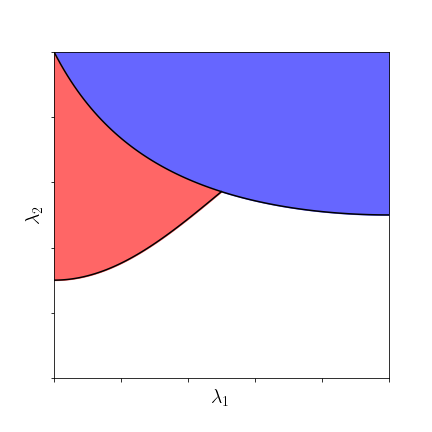
\includegraphics[width=0.28\columnwidth]{fake_phase_diagram.png}};
    \draw [->] (H.north) to[out=90,in=180] (A1.west);
    \draw [->] (H.south) to[out=-90,in=-180] (A2a.west);
    \draw [->] (A2a) -- (A2b);
    \draw [->] (A2b) -- (A2c);
    \draw [->] (A1) -- (B1);
    \draw [->] (A2c) -- (B2);
  \end{tikzpicture}
\end{center}

There could be other algorithms for this task taking an advantage of
quantum computers, but investigation of those is beyond the scope of this
paper.

There are 3 main challenges which need to be discussed before we can approach
specifying and solving this task.

\textbf{Issue 1: fixed finite size.}
One may observe, that we presented diagrams for fixed $L=10$ but wanted to
discuss phase transitions which are formally only defined in the thermodynamic
limit $L\to\infty$. That means, that one cannot see the actual phase transitions
on these diagrams, although one can see something which looks very close to
phase transitions: these are places where the color on these diagrams
changes quickly. Issue 1 is how to define the task of identifying
phase transitions for finite size Hamiltonians, where, strictly speaking,
there are no phase transitions due to finite fixed size.

\textbf{Issue 2: unknown order parameters.}
We want a method capable of identifying phase transitions in systems
for which these are not known yet. For those systems we may not know
what are the relevant order parameters. Issue 2 is how to define and
determine the phase transition in the absence of relevant known order parameters.

\textbf{Issue 3: loss of information at the time of measurement.}
ML algorithm only has access to bitstrings but, generally, bitstrings measured
in the computational basis do not contain
full information about the underlying quantum state.

There is a well-known approach \VK{TODO: cite} called fidelity susceptibility,
which we will use to address these issues. This is a quantity which
intuitively measures a squared rate of change of the underlying state.
By definition fidelity between two pure states $\ket{\phi}$ and $\ket{\psi}$ is
\begin{equation}
\label{eq:def.F.pure}
  F(\ket{\phi}, \ket{\psi}) = \abs{\braket{\phi\mid \psi}}.
\end{equation}
By definition fidelity between two mixed states
given by density matrices $\rho$ and $\sigma$ is
\begin{equation}
\label{eq:def.F.mixed}
  F(\rho, \sigma) = \Tr\left(\sqrt{\sqrt{\sigma}\rho\sqrt{\sigma}}\right).
\end{equation}
By definition classical fidelity between two discrete probability distributions
$p$ and $q$
\begin{equation}
\label{eq:def.Fc}
  F_c(p, q) = \sum_z \sqrt{p_z q_z}.
\end{equation}
In this paper we apply classical fidelity mainly to distributions over bitstrings
$z$ obtained from measurement in the computational basis of some quantum states.

Fidelity susceptibility $\chi_F(s)$ is defined when there is a state $\rho(s)$
depending on some parameter $s$. In this case we write $F(s_1, s_2)$ instead
of $F(\rho(s_1), \rho(s_2))$. Then
term in the Taylor expansion of the fidelity:
\begin{equation}
\label{eq:def.chiF}
  F(s, s + \delta s) = 1 - \frac{\delta s^2}{2} \chi_F(s) + o(\delta s^2).
\end{equation}
Similarly, the classical fidelity susceptibility $\chi_{F_c}(s)$ is defined by
\begin{equation}
\label{eq:def.chiFc}
  F_c(s, s + \delta s) = 1 - \frac{\delta s^2}{2} \chi_{F_c}(s) + o(\delta s^2).
\end{equation}

Issues 1 and 2 are then solved by defining the task we are trying to solve
as the task of identifying the local maxima of fidelity susceptibility.
To address issue 3 we look at the properties of the fidelity
susceptibility, its classical counterpart, and relations between them.

\subsection{Motivation for the definition of the task}
Finite size systems in the sequence of systems experiencing a phase transition
in the thermodynamic limit are known to often experience maxima of fidelity susceptibility at or around the location of the phase transition. Intuitively, that
makes sense because the fidelity susceptibility measures the square rate of change of the underlying state and it is known that phase transitions correspond to rapid change of the underlying state.

\subsection{Properties of fidelity susceptibility}
Roughly speaking, we plan to prove the following properties.
\begin{itemize}
  \item Formula \eqref{eq:def.F.mixed} is consistent with \eqref{eq:def.F.pure}
    for pure states and with \eqref{eq:def.Fc} for probability distributions.
  \item Usually, for fidelity susceptibility (or classical fidelity
    susceptibility) to be defined, only one derivative of wave function
    (or probabilities) needs to exist.
  \item $0 \leq \chi_{F_c}(s) \leq \chi_F(s)$.
  \item $\mathbb{E}_{\textrm{measurements}} \chi_{F_c}(s) = \chi_F(s)/2$.
  \item For non-degenerate ground states of real-valued Hamiltonians
  $\chi_{F_c}(s) = \chi_F(s)$ almost everywhere.
\end{itemize}
See the below theorems for the exact statements.
\VK{TODO: references to Zanardi papers: https://www.worldscientific.com/doi/abs/10.1142/S0217979210056335}

The following theorem states the properties of the fidelity relevant for this
paper. For proof of these, as well as many other, properties of the fidelity
the reader is referred to \cite[\S 9]{nielsen-chuang-2010}.
\begin{theorem}
  \begin{enumerate}
    \item If $\ket{\phi}$ and $\ket{\psi}$ are pure states, then
      \begin{equation}
        F(\ket{\phi}, \ket{\psi}) =
          F(\ket{\phi}\bra{\phi}, \ket{\psi}\bra{\psi}).
      \end{equation}
      In other words, \eqref{eq:def.F.pure} is consistent with
      \eqref{eq:def.F.mixed}.
    \item If $\rho$ and $\sigma$ are diagonal density matrices with diagonal
      entries equal to $\rho_{zz} = p_z$ and $\sigma_{zz} = q_z$ respectively, then
      \begin{equation}
        F(\rho, \sigma) = F_c(p, q).
      \end{equation}
      In other words, \eqref{eq:def.F.mixed} is consistent with \eqref{eq:def.Fc}.
    \item If $\rho$ and $\sigma$ are two density matrices, we have
      \begin{equation}
        \label{eq:prop.F.1}
        F(\rho, \sigma) = F(\sigma, \rho),
      \end{equation}
      \begin{equation}
        \label{eq:prop.F.2}
        0 \leq F(\rho, \sigma) \leq 1,
      \end{equation}
      \begin{equation}
        \label{eq:prop.F.3}
        F(\rho, \sigma) = 1 \textrm{ iff } \rho = \sigma,
      \end{equation}
      \begin{equation}
        \label{eq:prop.F.4}
        F(\rho, \sigma) = 0 \textrm{ iff } \rho \sigma = 0.
      \end{equation}
  \end{enumerate}
\end{theorem}

Before moving to fidelity susceptibility, we want to describe a generalization
of the fidelity susceptibility covered in \cite{zanardi2007information}.
Formulas \eqref{eq:def.chiF} and \eqref{eq:def.chiFc} assume dependence
on a single parameter $s$. In practice, the Hamiltonian of interest depends
on multiple parameters, e.g. the frustrated ladder Hamiltonian in
\eqref{eq:Hladder.1} depends on 3 real parameters: $s, K, U$. In general,
we can say that a state of interest depend on a parameter $\lambda$ from
a parameter manifold $\mathcal{M}$. In general, these parameters
can include the parameters of the Hamiltonian and the parameters impacting
how the state is derived from that Hamiltonian (e.g. temperature).
Then, similarly to equations
\eqref{eq:def.chiF} and \eqref{eq:def.chiFc} we can expand the fidelity
to the second order.
\begin{equation}
\label{eq:def.gF}
  F(\lambda, \lambda + \delta \lambda) =
  1 - \frac12 \sum_{\mu\nu} g_{\mu\nu} \delta \lambda^\mu \delta \lambda^\nu
  + o(\abs{\delta \lambda}^2).
\end{equation}
The resulting second term represents a metric
\begin{equation}
  \label{eq:def.gmetric}
  g = \sum_{\mu\nu} g_{\mu\nu} d\lambda^\mu d\lambda^\nu.
\end{equation}
The metric $g$ described by \eqref{eq:def.gF} and \eqref{eq:def.gmetric}
is invariant with
respect to the choice of the coordinates $\lambda$ on $\mathcal{M}$.
As explained in \cite{zanardi2007information}, phase transitions are expected
to correspond to singularities in the metric \eqref{eq:def.gmetric} in the
thermodynamic limit. We, however, are interested in the finite systems
of a fixed size. Therefore, we are interested in identifying the vectors
$\varphi$ on $\mathcal{M}$ with high values of
$g(\varphi, \varphi) / g_0(\varphi, \varphi)$,
where $g_0$ is a metric considered to be non-singular.
We also note that \eqref{eq:def.gmetric} is $1/4$ of Fisher Information Metric
for the case of classical fidelity when for all $z$ we have $p_z > 0$.

\begin{theorem}
  \label{th:def.g}
  \begin{enumerate}
    \item Suppose $\ket{\psi(\lambda)}$ is a state defined in the
      neighbourhood of
      $\lambda = \lambda_0 \in \mathcal{M}$ and differentiable at
      $\lambda=\lambda_0$.  Then the fidelity susceptibility metric
      is well-defined at
      $\lambda=\lambda_0$ and is given by
      \begin{multline}
        \label{eq:gmunu.pure}
        g_{\mu\nu}(\lambda_0) = \real\bigl(\braket{\partial_\mu \psi(\lambda_0)
          | \partial_\nu \psi(\lambda_0)}\bigr)\\
        - \braket{\partial_\mu \psi(\lambda_0) | \psi(\lambda_0)}
          \braket{\psi(\lambda_0) | \partial_\nu \psi(\lambda_0)},
      \end{multline}
      where $\partial_\mu \psi(\lambda_0)$ is a compact notation for the derivative
      $\left.\frac{\partial \psi(\lambda)}{\partial \lambda^\mu}
      \right|_{\lambda=\lambda_0}$.
    \item Suppose $\rho(\lambda)$ is a density matrix defined in the
      neighbourhood of $\lambda = \lambda_0 \in \mathcal{M}$, has the first
      derivative at $\lambda = \lambda_0$, and $\Tr(P_0 \rho(\lambda) P_0^{\dagger})$
      has the second derivative
      at $\lambda = \lambda_0$, where $P_0$ is the orthogonal
      projector $\mathcal{H} \to \ker\rho(\lambda_0)$.
      Let $P_{{+}}$ be the orthogonal projector
      $\mathcal{H} \to \rho(\lambda_0)(\mathcal{H})$,
      $\rho_{+}(\lambda) = P_{{+}} \rho(\lambda) P_{{+}}^{\dagger}$.
      Then in the basis where
      $\rho_{+}(\lambda_0) = \diag(\xi_0,\dots,\xi_{n_{+}})$
      we have
      \begin{multline}
        g_{\mu\nu}(\lambda_0)
        = \sum_{j,k} \frac{
            \real\left(
              (\partial_\mu\rho_{+}(\lambda_0))_{jk}
              (\partial_\nu\rho_{+}(\lambda_0))_{kj}
            \right)
          }{2(\xi_j + \xi_k)}\\
        + \frac12 \left.\partial_\mu \partial_\nu \Tr(P_0 \rho(\lambda) P_0^{\dagger})
          \right|_{\lambda=\lambda_0}.
      \end{multline}
      In that expression the second term can be bounded from below by
      \begin{equation}
        \label{eq:g2bound}
        \real\left(
          P_0 \left(\partial_\mu\rho(\lambda_0)\right)
          P_{+}^{\dagger} \left(\rho_{+}(\lambda_0)\right)^{-1}
          P_{+} \left(\partial_\nu\rho(\lambda_0)\right) P_0^{\dagger}
        \right).
      \end{equation}
      If the bound is not an equality along some vector $\phi$ tangent to
      $\mathcal{M}$ at $\lambda_0\in\mathcal{M}$ then $\rank(\rho(\lambda))$
      is larger than $\rank(\rho(\lambda_0))$ in some punctured neighbourhood
      of $\lambda_0$ (i.e. the neighbourhood
      excluding the point $\lambda_0$ itself) along the direction $\phi$.
    \item Suppose $p(\lambda) = \{p_z(\lambda)\}_{z \in \mathcal{S}}$
      is a discrete probability distribution on a finite set $\mathcal{S}$
      defined in a neighbourhood of $\lambda = \lambda_0 \in \mathcal{M}$.
      Let $\mathcal{S} = \mathcal{S}_{+} \cup \mathcal{S}_0$ be the split
      of $\mathcal{S}$ into subsets where $p_z(\lambda_0)$ is positive
      or zero respectively. Assume that $p_z$ has the first derivative
      at $\lambda = \lambda_0$ and $\sum_{z\in\mathcal{S}_0} p_z(\lambda)$
      has the second derivative at $\lambda = \lambda_0$. Then
      \begin{multline}
        \label{eq:gmunu.c}
        g_{\mu\nu}(\lambda_0) = \sum_{z\in\mathcal{S}_{+}}
        \frac{
          \left(\partial_{\mu} p_z(\lambda_0)\right)
          \left(\partial_{\nu} p_z(\lambda_0)\right)
        }{
          4 p_z(\lambda_0)
        } \\
        + \frac12 \left.\partial_{\mu} \partial_{\nu}
          \sum_{z\in\mathcal{S}_0} p_z(\lambda)\right|_{\lambda = \lambda_0}.
      \end{multline}
  \end{enumerate}
\end{theorem}
Part 1 of this theorem
is essentially the formula (3) in \cite{zanardi2007information}
with the exact conditions needed from $\ket{\varphi(\lambda)}$
specified. As mentioned in \cite{zanardi2007information},
the proof is essentially done by the Taylor expansion of \eqref{eq:def.F.pure}
and the usage of the fact that the Hilbert
space elements representing the states have the norm of 1. Since we do
not require the second derivative to exist, we have to do that expansion
with a bit more care than \cite{zanardi2007information}, as spelled out
in the proof below. Note also that part 2 is a generalization of part 1,
and the proof for part 2 won't use part 1, hence we could just leave
the proof for part 2. However, the proof for part 1 is much simpler,
so we leave it here.
\begin{proof}[Proof of part 1]
  Due to equivariance of the definition of $g_{\mu\nu}$ with respect to
  the change of the coordinates $\lambda \mapsto \lambda - \lambda_0$,
  without loss of generality we can prove the statements in the theorem for
  $\lambda_0 = 0$. Let $\ket{\psi_0} = \ket{\psi(0)}$,
  $\ket{\delta \psi} = \ket{\psi(\delta\lambda)} - \ket{\psi(0)}$.
  We know that
  \begin{equation}
    \ket{\delta \psi} = \sum_{\mu} \ket{\partial_\mu\psi(0)} \delta\lambda^\mu
      + \ket{r},
  \end{equation}
  where $\ket{r} = o(\abs{\delta\lambda})$.
  We also know that $\braket{\psi(\delta\lambda)|\psi(\delta\lambda)} = 1$.
  On the other hand,
  \begin{multline}
    \braket{\psi(\delta\lambda)|\psi(\delta\lambda)} =
    1 + 2\real{\braket{\psi_0|\delta\psi}} + \braket{\delta\psi|\delta\psi}\\
    = 1 + 2\sum_\mu\real{\braket{\psi_0|\partial_\mu\psi(0)}}\lambda^\mu
      + 2\real{\braket{\psi_0|r}}\\
      + \sum_{\mu,\nu}\braket{\partial_\mu\psi(0)|\partial_\nu\psi(0)}
        \delta\lambda^\mu \delta\lambda^\nu
      + o(\abs{\delta\lambda}^2).
  \end{multline}
  Thus,
  \begin{equation}
    \real{\braket{\psi_0|\partial_\mu\psi(0)}} = 0
  \end{equation}
  and
  \begin{multline}
    \real{\braket{\psi_0|r}} \\
      = - \frac12 \sum_{\mu,\nu}
        \braket{\partial_\mu\psi(0)|\partial_\nu\psi(0)}
        \delta\lambda^\mu \delta\lambda^\nu
    + o(\abs{\delta\lambda}^2).
  \end{multline}
  We compute
  \begin{multline}
    F(0, \delta\lambda) = \abs{\braket{\psi(0)|\psi(\delta\lambda)}}
    = \abs{1 + \braket{\psi_0|\delta \psi}} \\
    = \abs{1 + \sum_\mu\braket{\psi_0|\partial_\mu \psi(0)}\delta\lambda^\mu
      + \braket{\psi_0|r}} \\
    = 1 + \real{\braket{\psi_0|r}} - \frac12 \left(
      \sum_\mu\braket{\psi_0|\partial_\mu \psi(0)}\delta\lambda^\mu\right)^2\\
      + o(\abs{\delta\lambda}^2) \\
    = 1 - \frac12 \sum_{\mu\nu} g_{\mu\nu} \delta \lambda^\mu \delta \lambda^\nu
      + o(\abs{\delta \lambda}^2),
  \end{multline}
  where $g_{\mu\nu}$ is given by \eqref{eq:gmunu.pure}.
  Note that when expanding the absolute value we used
  the fact that for real $x,y$ around $x=y=0$ we have
  \begin{equation}
    \abs{1 + x + iy} = 1 + x + \frac{y^2}{2} + O(x^2 + y^4).
  \end{equation}
\end{proof}

\begin{lemma}
  \label{lm:block-diagonal}
  Let
  \begin{equation}
    M = \begin{pmatrix}A & B \\ B^{\dagger} & B^{\dagger} A^{-1} B + C\end{pmatrix}
  \end{equation}
  be a finite-dimensional block diagonal matrix over $\mathbb{C}$ with
  positive definite $A$.
  Then $M \geq 0$ iff $C \geq 0$.
  In that case $\rank(M) = \rank(A) + \rank(C)$.
\end{lemma}
\begin{proof}
  The lemma follows from the decomposition
  \begin{equation}
    M =
      \begin{pmatrix}A & B \\ 0 & 1\end{pmatrix}^{\dagger}
      \begin{pmatrix}A^{-1} & 0 \\ 0 & C\end{pmatrix}
      \begin{pmatrix}A & B \\ 0 & 1\end{pmatrix}.
  \end{equation}
\end{proof}

For part 2 see, e.g., \cite[section 15.1]{bengtsson_zyczkowski_2017}.
\begin{proof}[Proof of part 2]
  As in the previous proof, without loss of generality set $\lambda_0 = 0$.
  Denote $\rho_0 = \rho(0)$, $\delta \rho = \rho(\delta \lambda) - \rho_0$.
  We know that
  \begin{equation}
    \delta \rho = \sum_{\mu} \delta\lambda^\mu \partial_\mu\rho(0) + r,
  \end{equation}
  where $r = o(\abs{\delta \lambda})$. We also know that
  \begin{equation}
    \Tr\left(\partial_\mu\rho(0)\right) = 0,
  \end{equation}
  \begin{equation}
    \Tr(r) = 0.
  \end{equation}
  From definition,
  \begin{equation}
    F(\rho_0, \rho_0 + \delta \rho) =
    \Tr \sqrt{\rho_0^2 + \sqrt{\rho_0} \delta \rho \sqrt{\rho_0}}.
  \end{equation}
  Let $\rho_{0{+}} = P_{{+}} \rho_0 P_{{+}}^{\dagger}$,
  $\delta\rho_{+} = P_{{+}} \delta\rho P_{{+}}^{\dagger}$,
  $r_{+} = P_{{+}} r P_{{+}}^{\dagger}$. One can see that the expression under the
  square root acts nontrivially only on $\rho_0(\mathcal{H})$, hence the trace
  can be computed in that subspace:
  \begin{equation}
    \label{eq:F.Tr.sqrt}
    F(\rho_0, \rho_0 + \delta \rho) = \Tr \sqrt{
      \rho_{0{+}}^2 + \sqrt{\rho_{0{+}}} \delta \rho_{+} \sqrt{\rho_{0{+}}}
    }.
  \end{equation}
  For $\delta \lambda = 0$ the expression under the square root is equal to
  $\rho_{0{+}}^2$ and has only positive eigenvalues. Thus, for $\delta \lambda$
  in some neighbourhood of $0$ the spectrum of the expression under the square
  root lies in $(c_1, c_2)$ for some $c_1,c_2$ satisfying
  $0 < c_1 \leq c_2 < \infty$. Thus, in that neighbourhood the square root is
  an analytic function and can be expressed as an integral with the
  corresponding resolvent over a contour surrounding $[c_1, c_2]$:
  \begin{multline}
    \label{eq:oint}
    \sqrt{
      \rho_{0{+}}^2 + \sqrt{\rho_{0{+}}} \delta \rho_{+} \sqrt{\rho_{0{+}}}
    } \\
    = \frac{-1}{2\pi i} \oint \sqrt{z} \left(
      \rho_{0{+}}^2 + \sqrt{\rho_{0{+}}} \delta \rho_{+} \sqrt{\rho_{0{+}}} - z
    \right)^{-1} dz \\
    = I_0 + I_1 + I_2 + o(\abs{\delta \lambda}^2),
  \end{multline}
  where
  \begin{multline}
    I_k = \frac{(-1)^{k+1}}{2\pi i} \oint \sqrt{z}
    \left(\rho_{0{+}}^2 - z\right)^{-1}\\
    \left(\sqrt{\rho_{0{+}}} \delta \rho_{+} \sqrt{\rho_{0{+}}} \left(\rho_{0{+}}^2 - z\right)^{-1}\right)^{k} dz.
  \end{multline}
  In order to evaluate the metric, we only need to compute the diagonal elements
  of $I_0, I_1, I_2$ discarding any terms with order $o(\abs{\delta \lambda}^2)$.
  We pick the basis where $\rho_{0{+}}$ is diagonal with diagonal elements
  $\xi_0 \geq \xi_1 \geq \dots \geq \xi_{n_{+}-1} > 0$.
  \begin{equation}
    I_0 = \rho_{0{+}},
  \end{equation}
  \begin{equation}
    (I_1)_{jj} = \frac12 \delta \rho_{{+},jj}
    = \frac12 \sum_{\mu} \delta\lambda^{\mu} \partial_{\mu} \rho_{{+},jj}(0)
      + \frac12 r_{{+},jj},
  \end{equation}
  \VK{TODO: what is the proper way to separate ${+}$ and $jj$ in $r_{{+},jj}$?
  $(r_{+})_{jj}$, $r_{{+}jj}$, $r_{{+}\;jj}$?}

  To evaluate the diagonal entries of $I_2$ we note that for the contour
  \begin{center}
    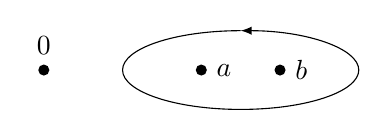
\begin{tikzpicture}
      \tikzstyle{bullet}=[circle, fill,minimum size=4pt, inner sep=0pt,
        outer sep=0pt];
      \draw (0, 0) node[style=bullet,label=90:$0$] {};
      \draw (2, 0) node[style=bullet,label=0:$a$] {};
      \draw (3, 0) node[style=bullet,label=0:$b$] {};
      \draw[-latex] (2.5, 0.5) arc (-270:90:1.5 and 0.5);
    \end{tikzpicture}
  \end{center}
  where $a,b$ are positive real numbers ($a$ could be equal to $b$),
  we have
  \begin{equation}
    \frac1{2\pi i} \oint \frac{\sqrt{z}}{(z-a)^2(z-b)} dz = \frac{-1}{2\sqrt{a}(\sqrt{a} + \sqrt{b})^2}.
  \end{equation}
  We then evaluate $(I_2)_{jj}$:
  \begin{multline}
    \label{eq:I2jj}
    (I_2)_{jj} = -\sum_k \frac{\xi_j \delta \rho_{{+},jk}
      \xi_k \delta \rho_{{+},kj}}{2\xi_j (\xi_j + \xi_k)^2}
    = -\sum_k \frac{\abs{\delta \rho_{{+},jk}}^2 \xi_k}{2(\xi_j + \xi_k)^2} \\
    = -\sum_{k,\mu,\nu} \frac{
        \real\left(
          (\partial_\mu\rho_{+}(0))_{jk}(\partial_\nu\rho_{+}(0))_{kj}
        \right) \xi_k
      }{2(\xi_j + \xi_k)^2} \delta\lambda^\mu\delta\lambda^\nu \\
      + o(\abs{\delta \lambda}^2).
  \end{multline}
  Now we are ready to evaluate the trace
  \begin{equation}
    F(\rho_0, \rho_0 + \delta \rho) =
      \Tr(I_0 + I_1 + I_2) + o(\abs{\delta\lambda}^2).
  \end{equation}
  In order to evaluate \eqref{eq:def.gF} we will include the terms up to
  the order $o(\abs{\delta \lambda}^2)$:
  \begin{equation}
    \Tr(I_0) = \Tr(\rho_0) = 1.
  \end{equation}
  The first term in $(I_1)_{jj}$ cannot have a non-zero contribution to
  $\Tr(I_1)$ due to the fact that $\rho(\lambda)$ is non-negative and
  has $\Tr(\rho(\lambda)) = 1$. For the second term, notice that $\Tr(r) = 0$,
  hence $\Tr(r_{+}) + \Tr(P_0 r P_0) = 0$, giving
  \begin{equation}
    \label{eq:TrI1}
    \Tr(I_1) = - \Tr(P_0 r P_0^{\dagger}) / 2.
  \end{equation}
  Note that according to lemma \ref{lm:block-diagonal}
  \begin{multline}
    P_0 r P_0^{\dagger}
    \geq \left(P_{+} \delta\rho P_0^{\dagger}\right)^{\dagger}
    \rho_{0{+}}^{-1} P_{+} \delta\rho P_0^{\dagger} \\
    = \sum_{\mu,\nu} \real\left(
        P_0 \left(\partial_\mu\rho(0)\right)
        P_{+}^{\dagger} \rho_{0{+}}^{-1}
        P_{+} \left(\partial_\nu\rho(0)\right) P_0^{\dagger}
      \right)
      \delta\lambda^\mu \delta\lambda^\nu \\
    + o(\abs{\delta \lambda}^2).
  \end{multline}
  Here $\real(a) = (a + a^{\dagger}) / 2$ for a matrix or an operator $a$.
  Combining \eqref{eq:I2jj} and \eqref{eq:TrI1} we get
  \begin{multline}
    g_{\mu\nu}(0)
    = \sum_{j,k} \frac{
        \real\left(
          (\partial_\mu\rho_{+}(0))_{jk}
          (\partial_\nu\rho_{+}(0))_{kj}
        \right) \xi_k
      }{(\xi_j + \xi_k)^2}\\
    + \frac12 \left.\partial_\mu \partial_\nu \Tr(P_0 \rho(\lambda)
    P_0^{\dagger}) \right|_{\lambda=0}.
  \end{multline}
  The remaining statements of the part 2 of the theorem follow from the
  lemma \ref{lm:block-diagonal}.
\end{proof}
Note that part 3 trivially follows from part 2 when applied to diagonal $\rho$.

\VK{The third term is weird.
Consider an example where $\mathcal{S} = \{0, 1\}$, $\mathcal{M} = \mathbb{R}$,
$p_0 = \sin^2(\theta)$, $p_1 = \cos^2(\theta)$. Then $g = (1 + \delta_{\sin(4\theta),0}) ds^2$.}

\begin{theorem}
  \label{th:avggc}
  Suppose $\ket{\psi(\lambda)}$ is a state defined in the
  neighbourhood of $\lambda = \lambda_0 \in \mathcal{M}$ and differentiable at
  $\lambda=\lambda_0$. Let $g$ be the corresponding fidelity metric
  and $g_c$ be its classical counterpart dependent on a projective
  measurement. then
  \begin{equation}
    \label{eq:Emeas}
    \mathbb{E}_{\textrm{measurements}} g_c(\lambda_0) = g(\lambda_0) / 2,
  \end{equation}
where the expectation $E_{\textrm{measurements}}$ is taken accross
all orthogonal bases in $\mathcal{H}$ using Haar measure (unique measure
invariant with respect to unitary rotations).
\VK{TODO: should ``measurements'' be italic in a formula inside a theorem?}
\end{theorem}
\begin{proof}
  The second term in \eqref{eq:gmunu.c} is only relevant when one of the
  vectors in the measurement basis is orthogonal to $\ket{\psi(\lambda_0)}$
  --- a subset of measure $0$ in the space of all measurements. Thus, we can
  safely discard it in \eqref{eq:Emeas}. To simplify the proof we notice that
  a quadratic form can be recovered from its values of the form
  $g(\lambda_0)(v, v)$,
  and both sides of the formula \eqref{eq:Emeas} are
  invariant with respect to the choice of coordinates.
  For a fixed $v$ we can always choose coordinates $\lambda$
  such that $v = \partial_0$, $\lambda_0 = 0$. It remains to prove that
  \begin{multline}
    \label{eq:Emeas.1}
    \mathbb{E}_{\textrm{measurements}}
    \sum_{z}
        \frac{
          \left(\partial_{0} p_z(0)\right)^2
        }{4 p_z(0)} \\
    = \frac12 \norm{\ket{\partial_{0} \psi(0)}}^2
        - \frac12 \abs{\braket{\partial_{0} \psi(0) | \psi(0)}}^2.
  \end{multline}
  One can simplify the l.h.s. by noting that the expectation of each term
  in the sum is the same. Thus, it remains to average over $\ket{\varphi}$
  s.t. $\norm{\ket{\varphi}} = 1$:
  \begin{multline}
    \textrm{l.h.s. of \eqref{eq:Emeas.1}}
    = n\mathbb{E}_{\ket{\varphi}}
      \frac{
        \left(\real\left(
        \braket{\varphi|\partial_{0} \psi(0)}
        \braket{\psi(0)|\varphi}\right)\right)^2
      }{\abs{\braket{\varphi|\psi(0)}}^2}.
  \end{multline}
  Let's denote
    $\ket{\psi_0} = \ket{\psi(0)}$,
    $\psi_\parallel = \braket{\psi_0|\partial_0\psi(0)}$,
    $\ket{\psi_\perp} = \ket{\partial_0\psi(0)} - \psi_\parallel\ket{\psi_0}$,
    $\varphi_\parallel = \braket{\psi_0|\varphi}$,
    $\ket{\varphi_\perp} = \ket{\varphi} - \varphi_\parallel\ket{\psi_0}$.
    Note that $\real(\psi_\parallel) = 0$.  With this notation
  \begin{equation}
    \textrm{r.h.s. of \eqref{eq:Emeas.1}} = \frac12 \norm{\ket{\psi_\perp}}^2,
  \end{equation}
  \begin{equation}
    \braket{\varphi|\partial_{0} \psi(0)} \braket{\psi(0)|\varphi} = 
    \abs{\varphi_\parallel}^2 \psi_\parallel
    + \varphi_\parallel \braket{\varphi_\perp|\psi_\perp}.
  \end{equation}
  Substituting this and averaging over arguments of $\varphi_\parallel$
  we get
  \begin{equation}
    \textrm{l.h.s. of \eqref{eq:Emeas.1}}
    = \frac{n}{2}\mathbb{E}_{\ket{\varphi}}
      \abs{\braket{\varphi_\perp|\psi_\perp}}^2
    = \frac12 \norm{\psi_\perp}^2.
  \end{equation}
\end{proof}

Given theorem \ref{th:avggc} is for pure states, one could wonder
whether a similar statement is true for mixed states. In general the answer
is negative. Moreover, it is possible to find a special case where
the average of the classical fidelity is 0 while the quantum fidelity
is non-zero:
\begin{equation}
  \rho(\lambda) =
    \begin{pmatrix}
      1 - \abs{\lambda}^2 & 0 \\
      0 & \abs{\lambda}^2
    \end{pmatrix}
\end{equation}
gives $g_{\mu\nu}(0) = 1$ while apart for one specific measurement basis where
one measures $\rho$ along the coordinates in which it is given
the classical fidelity is $0$ at $\lambda=0$ due to vanishing first derivatives.
Such extreme examples are rare. Indeed, the example relies on the bound
\eqref{eq:g2bound} not being an equality, hence the rank of $\rho$
being higher in the neighbourhood of a point where similar example applies
along the direction for which it applies. In one dimension that
a set of such values of $\lambda$ has to be discrete, in any number of
dimensions it has to have measure $0$.

In today's quantum annealer, though, the measurement basis is not random:
instead, there is a fixed basis called ``computational basis'' in which
all measurements are performed. At the same time, today's quantum annealers
have a limited set of biases and couplings allowed to the user. Below theorem
shows, that in this case too for pure states classical fidelity almost
everywhere is a good approximator of quantum fidelity. Even better, in this
case they are equal!
The main restriction on the Hamiltonian is that its matrix elements are
real, something which is true e.g. for $X$ and $Z$ biases,
and $XX$, $YY$, and $ZZ$ couplings.
\begin{theorem}
  \label{th:comput.basis}
  \begin{itemize}
    \item Suppose there is a continuously differentiable
      Hamiltonian $H(\lambda)$ acting on a
      finite-dimensional Hilbert space $\mathcal{H}$ with a basis which we
      will call ``computational basis''. Assume that matrix elements of the
      Hamiltonian are real in that basis. Also assume that the ground state of
      that Hamiltonian is non-degenerate.
      Then the ground state could be chosen to have real elements and
      continuously differentiable w.r.t. $\lambda$.
      elements.
    \item For a state differentiable w.r.t. $\lambda$ with real matrix elements,
      fidelity susceptibility metric coincides with its classical counterpart.
  \end{itemize}
\end{theorem}
\begin{proof}
  First, let's fix $\lambda$ and show that the ground state can be picked
  to be real for a Hamiltonian with real matrix elements.
  Indeed, let $\ket{\psi}$ be the ground
  state with ground energy $\epsilon_0$. We can represent it as
  \begin{equation}
    \ket{\psi} = \cos(\theta) \ket{\psi_0} + i\sin(\theta) \ket{\psi_1},
  \end{equation}
  where both $\ket{\psi_j}$ are normalized and have
  real vector elements, then we have
  \begin{multline}
    \epsilon_0 = \braket{\psi|H(\lambda)|\psi} \\
    = \cos^2(\theta) \braket{\psi_0|H(\lambda)|\psi_0}
      + \sin^2(\theta) \braket{\psi_1|H(\lambda)|\psi_1} \\
    \geq \epsilon_0 (\cos^2(\theta) + \sin^2(\theta))
    = \epsilon_0.
  \end{multline}
  Here the inequality is due to the fact that $\epsilon_0$ is the
  lowest energy level of $H(\lambda)$. Since it has to be an equality,
  we have
  \begin{equation}
    \braket{\psi_0|H(\lambda)|\psi_0} = \epsilon_0
      \textrm{ or } \cos(\theta) = 0,
  \end{equation}
  \begin{equation}
    \braket{\psi_1|H(\lambda)|\psi_1} = \epsilon_0
      \textrm{ or } \sin(\theta) = 0.
  \end{equation}
  Thus, at least one of $\psi_0$ or $\psi_1$ is the ground state
  with real vector elements.
  We can now finish the proof of part 1 by first applying implicit function
  theorem to $\det(H(\lambda) - \epsilon_0(\lambda))$ to show
  $\epsilon_0(\lambda)$ is differentiable, and then
  applying implicit function theorem to the system of equations obtained
  from $(H(\lambda) - \epsilon_0) \ket{\psi(\lambda)}$ by replacing
  one of the redundant rows with the equation
  \begin{equation}
    \norm{\ket{\psi(\lambda)}}^2 = 1.
  \end{equation}

  To prove the second part, notice that for the same reason as in the proof
  of theorem \ref{th:avggc}, it is sufficient to prove it for $g_{00}$.
  Then expanding both \eqref{eq:gmunu.pure} and \eqref{eq:gmunu.c} for
  a state with real vector elements, we get the same expression
  \begin{equation}
    g_{00}(\lambda) = \norm{\ket{\partial_0\psi(\lambda)}}^2.
  \end{equation}
\end{proof}

On the other hand, Hamiltonians with non-real matrix elements
can have $\chi_{F_c}(s) = 0$ with non-zero $\chi_F(s)$. For example,
consider
\begin{equation}
  H(s) = - (1-s) \sum_j X_j - s \sum_j Y_j.
\end{equation}
The eigenstate is $\ket{\psi(s)} = \ket{\psi_0(s)}^{\otimes n}$, where
\begin{equation}
  \ket{\psi_0(s)} = \frac1{\sqrt2} \left(
    \ket{0} + \frac{(1-s) + is}{\sqrt{1-2s(1-s)}}\ket{1}\right).
\end{equation}
These states generate uniform probability distribution independent of $s$
when measured in the computational basis. However, the state does change
with $s$, hence it has non-zero
\begin{equation}
  g(s) = \frac{n}{4} \left(d \arctan\left(\frac{s}{1-s}\right)\right)^2 =
  \frac{n\;ds^2}{4(1-2s(1-s))^2}.
\end{equation}

\subsection{Resolution of issue 3}
As we have seen in theorems \ref{th:avggc} and \ref{th:comput.basis},
classical fidelity susceptibility is expected to be between $\frac12 \chi_F(s)$
and $\chi_F(s)$ in many cases of interest. Thus, there is a hope that the
maximum of classical fidelity susceptibility would be close to the maximum
of fidelity susceptibility in cases of interest. In particular, the
Hamiltonians which could be implemented on the current quantum annealers are
stoquastic and, in particular, have real matrix elements in the computational
basis. Thus if the ground state is non-degenerate $\chi_{F_c}(s) = \chi_F(s)$
for the ground state and no information is lost when replacing $\chi_F(s)$ with
$\chi_{F_c}(s)$ if we are looking for phase transitions at zero temperature.
\VK{TODO: should we use here $g_c(s) = g(s)$? Should we then explain above
that we plan to use $g_c$ for classical fidelity susceptibility metric
whenever we want to avoid the ambiguity with the fidelity susceptibility?}

Thus, we can reformulate the setting of the paper as the challenge
between two approaches for identifying the maximums of $\chi_F(s)$.
The first approach is to use classical state of the art algorithms.
The second approach involves the following steps.
\begin{itemize}
  \item Use a quantum annealer to produce a dataset of pairs $(s,z)$,
    where $s$ is a value of the parameter and $z$ is a bitstring
    measured in the computational basis.
  \item Use an ML-based method, which we call Bitstring-ChiFc,
    to produce an estimate
    $\widehat\chi_{F_c}(s)$ of $\chi_{F_c}(s)$.
    See \VK{TODO} for the description of the method.
  \item Find local maxima $\hat s_{\textrm{critical},i}$ of the estimate.
  \item If necessary, refine the estimates $\hat s_{\textrm{critical}}$
    by repeating the algorithm with a smaller range of values of $s$
    around $\hat s_{\textrm{critical}}$.
\end{itemize}

Now we move to describe classical algorithms and their performance in this
task.

\subsection{Classical algorithm: Lanczos}
If we are interested in the fidelity suceptibility associated
to the ground states of the Hamiltonian, and the system size is small,
one of the powerful classical algorithms is based on Lanczos algorithm.
In the context of this algorithm we think about $H(\lambda)$ as
a sparse $2^n$ by $2^n$ matrix together with an algorithm to compute
$H(\lambda)\ket{\psi}$ for a vector $\ket{\psi}$ of the length $2^n$.
Typically, Hamiltonians we consider have
$\Theta(n)$ terms and the computation $H(\lambda)\ket{\psi}$
takes $\Theta(n2^n)$ time. Lanczos algorithm starts from
a random vector $\ket{\psi}$ and an integer $k$ (typically,
$k$ is of the order of 40). In exact arithmetic the algorithm would
return a unit vector $\ket{\varphi}$ from
$\mspan(\{H(\lambda)^j\ket{\psi}: j=0,\dots,k-1\})$
s.t. $\norm{\ket{\varphi}} = 1$ and $\braket{\varphi|H(\lambda)|\varphi}$
is the smallest possible. In practice, one performs the algorithm
using floating point numbers which causes an additional source of errors.
In fact, the Lanczos algorithm currently used in practice is different
from the one originally proposed by Lanczos, with most of the differences
intended to make the algorithm more resilient to numerical errors of
finite precision arithmetics while minimizing the additional computational
cost spent on these efforts.

One then would apply the algorithm for values of parameters on a grid
and estimate the fidelity susceptibility directly. E.g. if $H$ depends
on a single parameter $s\in[0,1]$ one could choose the number of points $N$
and compute $H(s)$ for $s\in\{j/N: j=0,\dots,N\}$, then estimate
\begin{equation}
  \hat \chi_F(s + \Delta s/2)
    \simeq 2 (1 - \abs{\braket{\varphi(s)| \varphi(s + \Delta s)}})
      / \Delta s^2,
\end{equation}
where $\Delta s = 1/N$, $s = j/N$, $j=0,\dots,N-1$.

The main downside of this approach is the need to perform $k$
multiplications of $H(\lambda)$ by a vector of size $2^n$, something
which typically takes time $\Theta(kn2^n)$, in each of $N$ executions
of the Lanczos algorithm. In practice, that means that
this method is the go to method for $n \leq 20$, being able to estimate
the fidelity to a good enough accuracy for $n=20$ in under 2 hours on a
single machine but impractical for $n > 40$.

There are cases where it fails due to either algorithmic or numerical issues,
especially if the gap between the ground state and first excited state is small,
or there is a large number of energy levels close to ground state energy.
However, in these cases other algorithms we reviewed would typically fail
as well and such failures could be easily detected by running the algorithm
with a different initial random state.

\subsection{Results}
Here is the comparison based on Lanczos diagonalization for L=10 (20-qubit)
frustrated ladder Hamiltonian with $K=U=1$: ground truth from Lanczos
vs reconstruction from Bitstring-ChiFc method.
\begin{center}
  \pgfmathparse{\columnwidth/20.79cm}%
  \edef\tikzscale{\pgfmathresult}%
  \begin{tikzpicture}[scale=\tikzscale, every node/.style={scale=\tikzscale}]
    % Bitstring-ChiFc: Lanczos (almost exact) vs our method (estimate).
    \draw (0, 0) node {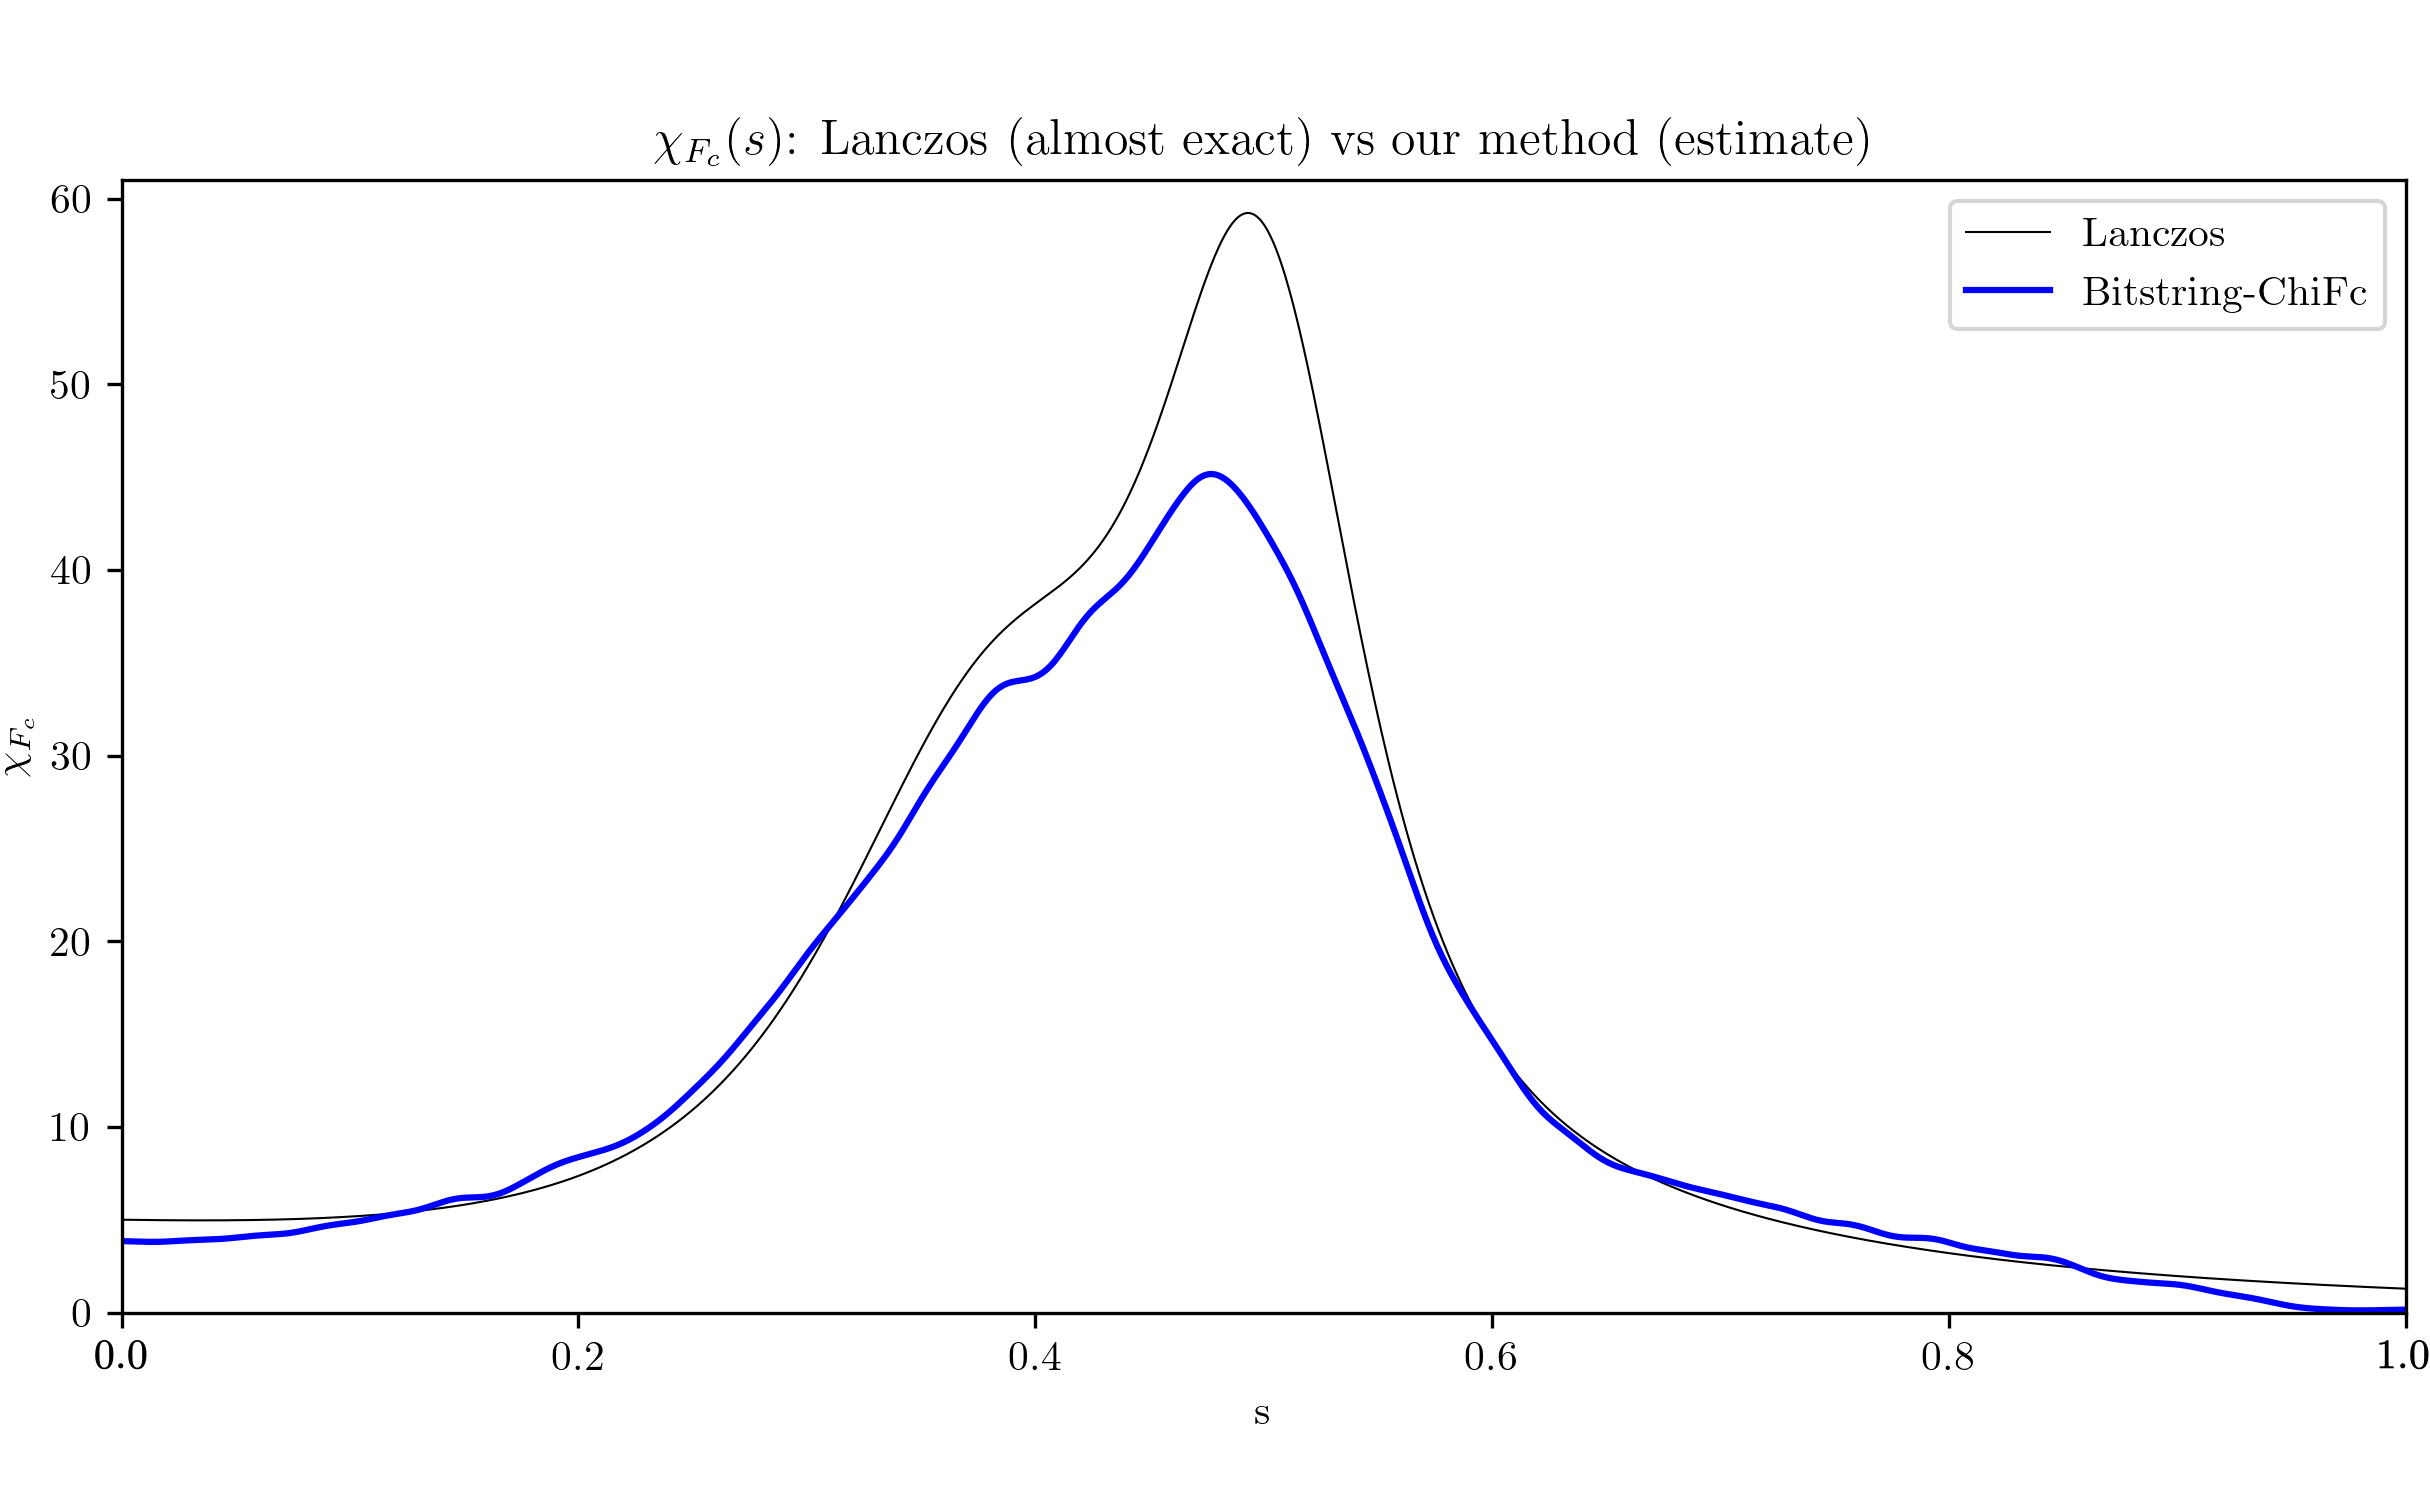
\includegraphics{ladder-ed-chifc.png}};
    \draw[blue, line width=0.4mm] (-0.05, -4.8) -- (-0.05, 4.8);
    \draw (0.28, -4.8) -- (0.28, 4.8);
    \draw (-2.3, -3.9) node[align=right] {predicted\\phase transition\\(using 140140 bitstrings)};
    \draw (1.75, -3.9) node[align=left]{actual\\phase transition};
    \draw (-1.7, 3) node[align=center]
    {$\uparrow\uparrow\uparrow\uparrow\downarrow\uparrow\downarrow\downarrow\downarrow\downarrow$\\
    $\uparrow\downarrow\uparrow\downarrow\downarrow\downarrow\downarrow\downarrow\downarrow\downarrow$};
    \draw (2.2, 3) node[align=center]
    {$\downarrow\uparrow\downarrow\uparrow\downarrow\uparrow\downarrow\uparrow\downarrow\uparrow$\\
    $\downarrow\downarrow\downarrow\downarrow\downarrow\downarrow\downarrow\downarrow\downarrow\downarrow$};
  \end{tikzpicture}
\end{center}

\section{TODO}
\begin{enumerate}
\item Complete presentation section above.
\item Write down the proofs for the fidelity susceptibility claims below.
\item Describe the models and practical results for them.
\end{enumerate}

\section{Introduction}
TODO:

Such a family can arise, e.g., from measurements of a low-temperature
Gibbs ensemble of Hamiltonians parametrized by a parameter $\lambda$.

\section{Classical Fidelity Susceptibility}
Classical fidelity between 2 probability distributions $p$ and $q$ of
bitstrings $z$ is defined as
\begin{equation}
  F_c(p, q) = \sum_{z} \sqrt{p(z) q(z)}.
\end{equation}
We are interested in the fidelity between bitstring distributions at different
$s$ (e.g. $s=s_1$ and $s=s_2$), which we will denote as $F_c(s_1, s_2)$.

\NE{This is an example of a commonly used in-line comment which is separated by color. I could say something like: "This sentence is awkward" or "Needs citation" or very meta "Please use enquote for real quotes and not literal quotes."}

Fidelity susceptibility is defined as the term $\chi_{F_c}(s)$ in the Taylor
expansion
\begin{equation}
\label{eq:Fcs.Tailor}
  F_c(s, s+\delta s) = 1 - \frac{\delta s^2}{2} \chi_{F_c}(s) + O(\delta s^3).
\end{equation}
For such Taylor expansion to exist it is sufficient that the probabilities have
a Taylor expansion up to $O(\delta s^3)$. More generally, probability
distribution can depend on a point $\lambda$ on a manifold $\Lambda$,
in which case the Tailor expansion \eqref{eq:Fcs.Tailor} would become
\begin{equation}
\label{eq:Fcl.Tailor}
  F_c(\lambda, \lambda+\delta \lambda) = 1 - \frac{\delta \lambda_{j} \delta \lambda_k}{2} \chi_{F_c}^{jk}(\lambda) + O(\delta \lambda^3).
\end{equation}

\subsection{Classical and quantum fidelity susceptibility}
Fact 1: For pure states $\mathbb{E}\chi_{F_c} (s) = \frac12 \chi_F (s)$
where the expectation is over all orthogonal bases to perform the measurement in.

TODO:proof

Fact 2: For computational basis measurement of a non-degenerate ground state
of a real-valued Hamiltonian $H$, then $\chi_{F_c}(s) = \chi_F(s)$
almost everywhere.

TODO:proof

\section{Problem setup}
\begin{itemize}
  \item In this work we consider a family of distributions of
bitstrings $\{\mathcal{D}_{\lambda}\}_{\lambda \in \Lambda}$, each of length $n$.
  \item We are given a finite sample $\mathcal{D}_{\textrm{train}}$ of size $N$
  of pairs $(\lambda, z)$ s.t. $P(z|\lambda) = P_{\mathcal{D}_{\lambda}}(z)$.
  \item We are also given (possibly implicitly via coordinate description of $\Lambda$) a naive metric $g^0$ on $\Lambda$.
  \item We are asked to estimate the Fisher information metric $g$ on $\Lambda$ corresponding to distributions $\mathcal{D}_{\lambda}$.
  \item Locations with high $g / g^0$ are then considered to be conjectured locations of possible phase transitions.
\end{itemize}

We focus on the task of identifying phase transitions in that
family. Rigorously speaking, phase transitions are only defined
in the limit $n\to\infty$, while we are dealing with finite size systems.
A solution to that is to look at Fisher information metric: high distances according to Fisher information metric for points close according to naive metric likely correspond to phase transitions.

\section{Bitstring-ChiFc method}
In this work we propose the following method:
\begin{itemize}
  \item Collect a training dataset
  \begin{equation}
    \mathcal{D}_{\chi_{F_c}\textrm{-train}} = \{(\lambda_0, \delta \lambda, z, y),\dots\},
  \end{equation}
  where $z$ is sampled from
  $p(\bullet, \lambda=\lambda_{z})$,
  $p_{+} = p(\lambda_{z} = \lambda_0 + \delta \lambda / 2| \lambda_{z} = \lambda_0 \pm \delta \lambda / 2)$, and
    $\mathbb{E}(y|\lambda_0, \delta \lambda, z) = p_{+}$.
    In practice $y \in \{0, 1\}$.
    Do it in the following way:
    \begin{itemize}
      \item Consider $\mathcal{D}_{\textrm{train}}$ consisting of pairs
      $(z, \lambda)$.
      \item Sample pairs $(z_{i{+}}, \lambda_{i{+}})$,
      $(z_{i{-}}, \lambda_{i{-}})$ from $\mathcal{D}_{\textrm{train}}$.
      \item Compute $\lambda_i = (\lambda_{i{+}} + \lambda_{i{-}})/2$,
      $\delta \lambda_i = \lambda_{i{+}} - \lambda_{i{-}}$.
      \item Add tuples $(\lambda_i, \delta \lambda_i, z_{i{+}}, 1)$ and $(\lambda_i, \delta \lambda_i, z_{i{-}}, 0)$ to the dataset $\mathcal{D}_{\chi_{F_c}\textrm{-train}}$.
    \end{itemize}
  \item Train a model $M$, which given $(\lambda_0, \delta \lambda, z)$
  will predict $l = M(\lambda_0, \delta \lambda, z)$
  s.t. $p_{+} = (1+e^{-l \cdot \delta \lambda})^{-1}$.
  Do this by minimizing cross-entropy loss on the dataset
  $\mathcal{D}_{\chi_{F_c}\textrm{-train}}$.
  \item Estimate
  \begin{multline}
  \label{eq:chifc-from-M}
  \left(\hat g_{c}\right)_{\mu\nu}(\lambda) = \smoothen\Bigl(
  \lambda_1 \mapsto \mean_{(z, \lambda_1) \in \mathcal{D}_{\textrm{train}}}
  \bigl(\\
  M(\lambda_1, 0, z)_{\mu}M(\lambda_1, 0, z)_{\nu}\bigr)\Bigr)(\lambda).
  \end{multline}
\end{itemize}

\subsection{Justification for the formula for Bitstring-ChiFc method.}
Here we justify the formula used for Bitstring-ChiFc
method.
\begin{theorem}
    Assume that the model $M$ is continuous with respect to
    $\delta \lambda$ and
    has the best possible out of sample performance
    near $\delta \lambda = 0$.
    Then
    \begin{equation}
      \label{eq:chifc-from-M-perfect}
      \left(g_{c}\right)_{\mu\nu}(\lambda) =
        \mathbb{E}_{(z, \lambda) \in \mathcal{D}}
        \left(
          M(\lambda, 0, z)_{\mu}M(\lambda, 0, z)_{\nu}
        \right).
    \end{equation}
\end{theorem}
In some sense the theorem justifies the use of formula
\eqref{eq:chifc-from-M}: it essentially shows that if the model
is perfect, and the dataset used in \eqref{eq:chifc-from-M} is
infinite, then that formula \eqref{eq:chifc-from-M} without the
smoothing gives a perfect estimate for the classical fidelity
susceptibility metric $g_c$. Of course, in reality these assumptions are not realistic: the model is not perfect, the dataset is finite, and the smoothing is necessary to dampen high frequency noise arising from the finite dataset size.
\VK{TODO: Should we discuss the imperfections
in a later subsection?}
\begin{proof}
  Both lhs and rhs of \eqref{eq:chifc-from-M-perfect} are 
  quadratic forms equivariant under the rotations of the 
  coordinate system of the parameter space. Therefore,
  it is sufficient to show they are equal for $\mu = \nu = 0$.
  That is, it is sufficient to prove the theorem in the scalar 
  case, where $\lambda$ consists of a single parameter $s$.
  In this case \eqref{eq:chifc-from-M-perfect} takes the form
  \begin{equation}
      \label{eq:chifc-from-M-perfect-s}
      \chi_{F_c}(s) =
        \mathbb{E}_{(z, s) \in \mathcal{D}} \left(
        M(s, 0, z)^2\right).
  \end{equation}
  By definition \eqref{eq:def.chiFc} and \eqref{eq:def.Fc} we
  have
  \begin{multline}
    \chi_{F_c}(s) = \lim_{\delta s \to 0} \frac{2}{\delta s^2}
    \Biggl(\\
      1-\sum_{z} \sqrt{P(z|s - \delta s / 2) P(z|s+\delta s/2)}
    \Biggr).
  \end{multline}
  Let's introduce the distribution $Q$ on bitstrings $z$
  by $Q(z) = (P(z|s - \delta s / 2) + P(z|s+\delta s/2)) / 2$.
  \VK{TODO:0 == Work in progress: START}
\end{proof}
Then we show that under these (unrealistic) assumptions
the formula \eqref{eq:chifc-from-M}
without the smoothing part produces the perfect estimate for $\chi_{F_c}$.
By definition, we have

\VK{TODO:2: expand the explanation for $s$ instead of $\lambda$.}

    \begin{multline*}
      \chi_{F_c}(\lambda) = \lim_{\delta \lambda\to 0} \frac2{\delta \lambda^2} \left(1 - \mathbb{E}_{z\sim Q(\bullet)} \frac{\sqrt{P(z|\lambda-\delta \lambda/2)P(z|\lambda+\delta \lambda/2)}}{Q(z)}\right)
      \\ \simeq \lim_{\delta \lambda\to 0} \mathbb{E}_{Q}\frac2{\delta \lambda^2}\frac{2\sinh^2(l\delta \lambda/4)}{\cosh(l\delta \lambda/2)} \simeq \frac14 \mathbb{E}_{z|\lambda} M(\lambda, 0, z)^2.
    \end{multline*}

TODO: models

TODO: experiments

\VK{TODO:2: 2nd part of the presentation with an image: presentation is a more low-low hanging fruit.}
\VK{Work in progress: END}

\bibliography{biblio.bib}
\bibliographystyle{apsrev4-1}

\end{document}
